\chapter{Konzeption des Systems und der Datenaufbereitung}
\label{ch:konzept}

\section{Methodisches Vorgehen}
\label{sec:methodisches_vorgehen}
\paragraphheading{Untersuchungsphasen und Nachweisführung}

Ausgangspunkt der Untersuchung sind die Forschungsfragen aus
Abschnitt~\ref{sec:zielsetzung} und die aus der Datengrundlage abgeleiteten
Anforderungen in Abschnitt~\ref{sec:anforderungskatalog}. Das methodische
Vorgehen gliedert sich darauf aufbauend in Konzeption, prototypische Umsetzung
und Prüfung. In der Konzeptionsphase werden zunächst die Verfahren anhand der
Anforderungen ausgewählt und zu einer Verarbeitungskette mit definierten
Ein- und Ausgaben verbunden. Dabei wird zwischen vorab festgelegten
Randbedingungen und Parametern unterschieden, die anhand der Trainingsgruppe
bestimmt werden. Anschließend wird das Evaluationsvorgehen festgelegt.

Die prototypische Umsetzung verbindet die einzelnen Softwarekomponenten zu
einer ausführbaren Pipeline. Die Implementierung wird in
Kapitel~\ref{ch:implementierung} beschrieben.

Die Prüfung erfolgt auf Komponenten- und Systemebene.

Auf Komponentenebene wird die Signaltrennung mit synthetischen Signalen
bekannter Zusammensetzung untersucht. Die Implementierung des Fast Kurtogram
wird mit einer separat ausgeführten Referenzimplementierung in MATLAB
verglichen. Beide Verarbeitungsschritte werden damit unabhängig von der
abschließenden Fehlerindikation geprüft.

Auf Systemebene werden die ausgewählten Messungen mit der vollständigen
Pipeline vom Datenimport bis zur Fehlerindikation verarbeitet. Die dabei
erzeugten Fehlerindikationen werden mit den dokumentierten Referenzklassen
verglichen.

Die Durchführung und die Ergebnisse der Versuche werden in
Kapitel~\ref{ch:evaluation} dargestellt und bewertet.

\paragraphheading{Trennung von Parametrierung und Evaluation}

Wie in Abschnitt~\ref{sec:untersuchungsrahmen} beschrieben, dienen die
Paderborner Trainingsdaten zur Auswahl der Analyse- und
Entscheidungsparameter. Die Paderborner Evaluationsdaten und die CWRU-Daten
werden erst anschließend verwendet, um die festgelegte Konfiguration zu
bewerten.

Die Parametersuche erhält ausschließlich die als Trainingsdaten ausgewählten
Paderborner Messungen. Nach ihrem Abschluss laden die Evaluationsskripte die
nach der Rangfolge in Abschnitt~\ref{sec:parametrierungsstrategie} ausgewählte
Konfiguration. Sie wenden deren Analyse- und Entscheidungsparameter ohne
erneute Auswahl auf die Paderborner Evaluationsdaten und die CWRU-Daten an.
Abtastrate, Lagergeometrie und Datenimport sind davon getrennte Angaben, die
für das Einlesen und Verarbeiten der jeweiligen Messung benötigt werden. Der
bekannte Zustand einer Evaluationsmessung wird erst nach der Verarbeitung mit
der Ausgabe der Pipeline verglichen. Er wird nicht als Eingang an die
Pipeline übergeben und nicht für die Parameterwahl verwendet.

Die Tests einzelner Komponenten sind davon zu unterscheiden. Bei ihnen dürfen
bekannte synthetische Signalbestandteile oder numerische Referenzausgaben
verwendet werden, um die Implementierung zu prüfen. Diese bekannten Werte
dienen nur dem jeweiligen Komponententest und nicht der Auswahl der später
bewerteten Parameterkonfiguration.

\section{Methodenauswahl}
\label{sec:methodenauswahl}

\paragraphheading{Auswahlkriterien}

Die Verfahren werden nicht allgemein bewertet. Sie werden passend zu den
Forschungsfragen, den ausgewählten Datensätzen und den Anforderungen an den
Prototyp ausgewählt. Zusätzlich wird berücksichtigt, ob sich ein Verfahren mit
den verfügbaren Daten, der vorhandenen Softwareumgebung und dem zeitlichen
Rahmen der Arbeit umsetzen und prüfen lässt. Dabei werden sowohl der
Implementierungsaufwand als auch der Rechenaufwand betrachtet. Die
Eingangsschnittstelle muss das Schwingungssignal, die zugehörige Abtastrate und
Drehzahl sowie die Lagergeometrie bereitstellen. Die abschließende
Fehlerindikation muss sich auf die betrachteten Innen- und Außenringschäden
beziehen lassen. Der Weg von der Messung bis zu dieser Indikation muss
nachvollziehbar sein. Signaltrennung, Bandauswahl und Fehlerindikation müssen
gemäß F-03 getrennt prüfbar und gemäß Q-01 als getrennte
Pipelinekomponenten nutzbar sein.

Die Methodenkette muss für Messungen aus beiden Referenzdatensätzen nutzbar
sein. Die Referenzklasse darf dabei nicht in die Signalverarbeitung oder
Fehlerindikation eingehen. Unterschiede beim Datenimport, bei der Abtastrate
und bei der Lagergeometrie müssen an der Eingangsschnittstelle behandelt
werden. Danach sollen die Messungen dieselben Verarbeitungsschritte
durchlaufen. Parameter, die anhand der Referenzklassen optimiert werden,
dürfen ausschließlich anhand der Paderborner Trainingsgruppe bestimmt werden.
Auswahl, Parametrierung und spätere Bewertung bleiben damit klar getrennt.

\paragraphheading{Auswahl der Signaltrennung}

Ziel der Signaltrennung ist es, stabile deterministische Signalanteile vor der
Hüllkurvenanalyse zu entfernen und die stochastischen beziehungsweise
pseudo\-zyklo\-stationären Lageranteile für die nachfolgende Analyse zu
erhalten. Für die Auswahl sind vor allem die benötigten Eingangssignale, der
Umfang der Trennung, der Einstellungsaufwand und der Rechenaufwand relevant.

Die Grundlagen der verglichenen Verfahren sind in
Abschnitt~\ref{sec:signalseparation} erläutert.

Die \gls{TSA} mittelt Signalabschnitte, die jeweils einer Periode der
betrachteten periodischen Komponente entsprechen. Damit die Abschnitte trotz
kleiner Drehzahlschwankungen derselben Winkelposition zugeordnet werden können,
wird das Signal zunächst winkeläquidistant neu abgetastet. Das Order Tracking
stellt zugleich sicher, dass der erste Abtastwert
jeder Periode einem bestimmten Phasenwinkel der Periodizität entspricht. Die
winkeläquidistante Neuabtastung basiert üblicherweise auf einem Referenzsignal
eines Tachometers oder Encoders
\cite[S.~11--12, Abschn.~2]
{randallComparisonMethodsSeparation2011}.
Die Mittelung extrahiert den Signalanteil mit der ausgewählten Periode. Für
jede weitere periodische Komponente beziehungsweise Harmonischenfamilie muss
die TSA separat durchgeführt werden. Dabei entfernt sie die Harmonischen der
jeweiligen Familie, jedoch keine Modulationsseitenbänder
\cite[S.~11, Abschn.~2; S.~18, Abschn.~7]
{randallComparisonMethodsSeparation2011}.

Die lineare Prädiktion arbeitet direkt mit dem Messsignal. Sie bildet aus
vorangegangenen Signalwerten ein Modell des vorhersagbaren und damit
deterministischen Anteils. Die Modellordnung beeinflusst, welche
deterministischen Frequenzanteile entfernt werden
\cite[S.~13--14, Abschn.~3]
{randallComparisonMethodsSeparation2011}.

Die \gls{ANC} benötigt dagegen ein separat gemessenes Referenzsignal, das mit
der zu entfernenden Komponente kohärent ist, sodass beide durch eine lineare
Übertragungsfunktion zusammenhängen. Der adaptive Filter bestimmt diese
Übertragungsfunktion und subtrahiert das entsprechend angepasste
Referenzsignal vom Eingangssignal, sodass der andere Signalanteil verbleibt
\cite[S.~183, Abschn.~5.3.3]
{randallVibrationbasedConditionMonitoring2022}.
Bei der \gls{SANC} wird das zusätzliche Referenzsignal durch eine verzögerte
Kopie des Eingangssignals ersetzt. SANC kommt daher mit einem Messsignal aus.
Für die Anwendung müssen jedoch Verzögerung, Filterordnung und
Konvergenzfaktor festgelegt werden
\cite[S.~184--185, Abschn.~5.3.4]
{randallVibrationbasedConditionMonitoring2022}.
\gls{DRS} nutzt ebenfalls das Signal und eine verzögerte Kopie, bestimmt den
Trennfilter jedoch im Frequenzbereich. Im Gegensatz zu SANC wird der Filter
zunächst aus den Daten bestimmt und anschließend auf dieselben Daten
angewandt; eine adaptive Anpassung entfällt
\cite[S.~185--186, Abschn.~5.3.5]
{randallVibrationbasedConditionMonitoring2022}.

Auch das cepstrale Editieren benötigt nur das zu untersuchende Signal. Das
Verfahren entfernt gezielt ausgewählte Harmonischen- und Seitenbandgruppen.
Damit lassen sich bestimmte vorgegebene periodische Familien entfernen,
während andere beibehalten werden
\cite[S.~17--18, Abschn.~6--7]
{randallComparisonMethodsSeparation2011}.

Tabelle~\ref{tab:entscheidung_signaltrennung} bewertet die für die Pipeline
entscheidenden Eigenschaften. Die Verfahrenseigenschaften beruhen auf den in
Abschnitt~\ref{sec:signalseparation} dargestellten Quellen; Gewichtung und
Punktvergabe sind eine eigene methodische Bewertung. Ein Kriterium erhält 0
Punkte, wenn es nicht erfüllt ist, 1 Punkt bei teilweiser Erfüllung und 2
Punkte bei vollständiger Erfüllung. Der Nutzwert ergibt sich aus der Summe der
gewichteten Bewertungen; maximal sind 24 Punkte erreichbar.

\begin{table}[H]
  \centering
  \caption{Entscheidungsmatrix der Trennverfahren (eigene Bewertung)}
  \label{tab:entscheidung_signaltrennung}
  \small
  \renewcommand{\arraystretch}{1.15}
  \begin{tabularx}{\textwidth}{|>{\raggedright\arraybackslash}X|c|*{6}{>{\centering\arraybackslash}p{0.95cm}|}}
    \hline
    \textbf{Kriterium} & \textbf{Gewicht} & \textbf{TSA} &
    \textbf{Lin. Präd.} & \textbf{ANC} & \textbf{SANC} &
    \textbf{\shortstack{Cep-\\stral}} & \textbf{DRS} \\
    \hline
    Kein zusätzliches Referenzsignal erforderlich
    & 3 & 0 & 2 & 0 & 2 & 2 & 2 \\
    \hline
    Alle deterministischen Komponenten werden gemeinsam entfernt
    & 3 & 0 & 1 & 1 & 2 & 1 & 2 \\
    \hline
    Zu entfernende Komponenten müssen nicht vorher festgelegt werden
    & 2 & 0 & 1 & 0 & 2 & 0 & 2 \\
    \hline
    Geringer Einstellungsaufwand
    & 2 & 1 & 0 & 0 & 0 & 1 & 2 \\
    \hline
    Geringer Rechenaufwand bei vielen deterministischen Komponenten
    & 2 & 0 & 1 & 0 & 1 & 1 & 2 \\
    \hline
    \textbf{Nutzwert} & -- & \textbf{2} & \textbf{13} & \textbf{3} &
    \textbf{18} & \textbf{13} & \textbf{24} \\
    \hline
  \end{tabularx}
\end{table}

Die beiden am höchsten gewichteten Kriterien betreffen die verfügbaren
Eingangsdaten und das Trennziel. Die gemeinsame Pipeline erhält kein
Tachometer-, Encoder- oder sonstiges Referenzsignal. Deshalb sind TSA und ANC
ohne eine Erweiterung der Eingangsschnittstelle nicht allgemein anwendbar.
Bei TSA kommt hinzu, dass jede Periodizität separat behandelt werden muss. Bei
ANC legt das bereitgestellte Referenzsignal fest, welcher kohärente Anteil
entfernt wird.

Lineare Prädiktion und cepstrales Editieren können mit einem Messsignal
arbeiten. Die lineare Prädiktion erfordert jedoch die Wahl einer geeigneten
Modellordnung. Beim cepstralen Editieren müssen die zu entfernenden
periodischen Anteile vorab ausgewählt werden. Beide Verfahren sind daher
weniger gut für eine gemeinsame, weitgehend automatisch arbeitende Pipeline
geeignet.

SANC erreicht den zweithöchsten Nutzwert. Das Verfahren entfernt die
deterministischen Komponenten einschließlich ihrer Seitenbänder, ohne dass ein
zweiter Messkanal benötigt wird. Der Filter muss sich jedoch schrittweise
anpassen. Für mechanische Systeme kann dabei eine Filterordnung von mehreren
Hundert oder Tausend erforderlich sein. Der Konvergenzfaktor muss so gewählt
werden, dass weder Divergenz noch eine übermäßig lange Anpassungszeit auftritt
\cite[S.~184--185, Abschn.~5.3.4]
{randallVibrationbasedConditionMonitoring2022}.
Antoni und Randall berichten zudem von Konvergenzproblemen, durch die das
gleiche Signal teilweise mehrfach verarbeitet werden musste
\cite[S.~104, Abschn.~1]
{antoniUnsupervisedNoiseCancellation2004}.

DRS erreicht mit 24 Punkten den höchsten Nutzwert. Es arbeitet ebenfalls mit
einem Messsignal und entfernt die stabilen deterministischen Komponenten
gemeinsam, ohne dass diese vorher einzeln festgelegt werden müssen. Der Filter
wird im Frequenzbereich bestimmt. Gegenüber SANC erzielt DRS ein vergleichbares
Trennergebnis mit geringerem Rechenaufwand und ohne Divergenzrisiko
\cites[S.~103--105, Abschn.~1--2]
{antoniUnsupervisedNoiseCancellation2004}
[S.~185--186, Abschn.~5.3.5]
{randallVibrationbasedConditionMonitoring2022}.
Damit ist DRS für die gemeinsame Pipeline am besten geeignet. Das für die
weitere Analyse verwendete Residuum entsteht, indem der ermittelte
deterministische Anteil vom Eingangssignal abgezogen wird.

Für die Offline-Auswertung wird die in Abschnitt~\ref{sec:signalseparation}
erläuterte amplitudenbasierte Filterung mit $\lvert H_1(f)\rvert$ gewählt.
Sie verändert die Phase der durchgelassenen Komponenten nicht und ist
nichtkausal
\cite[S.~15, Abschn.~5]{randallComparisonMethodsSeparation2011}.
Da die Messreihen vor der Verarbeitung vollständig vorliegen, ist für diese
Arbeit kein kausaler Filter erforderlich. Die Variante ermöglicht damit die
Signaltrennung ohne eine zusätzliche Phasenkorrektur des komplexen Filters.

Diese Auswahl setzt voraus, dass die deterministischen Signalanteile während
einer Aufzeichnung hinreichend stabil bleiben. Bei stärkeren
Drehzahlschwankungen wäre vor der Trennung ein Order Tracking, also eine
Neuabtastung mit konstanten Winkelabständen, erforderlich
\cite[S.~18]{randallComparisonMethodsSeparation2011}. Die Paderborner
Messungen wurden innerhalb einer Aufzeichnung bei konstanten Betriebsgrößen
durchgeführt; auch die CWRU-Versuche weisen innerhalb eines Versuchs eine
konstante Drehzahl auf
\cites[S.~8, Abschn.~4.2 und Tab.~6]
{lessmeierConditionMonitoringBearing2016}
[S.~102--103, Abschn.~3.1]
{smithRollingElementBearing2015}.
Ob die Stabilität im Einzelfall ausreicht, wird dennoch erst durch die
Evaluation geprüft. Dazu wird jede Messung einmal mit DRS und einmal ohne
Signaltrennung verarbeitet. In der zweiten Variante werden Bandauswahl,
Hüllkurvenanalyse und Fehlerindikation unmittelbar auf das Rohsignal
angewandt. Der Vergleich beider Varianten ermöglicht eine getrennte Bewertung
des Beitrags der Signaltrennung.

\paragraphheading{Auswahl des Frequenzbandes}
\label{par:auswahl_frequenzband}

Für die Hüllkurvenanalyse muss vor der Demodulation das auszuwertende
Frequenzband festgelegt werden. Ein datensatzübergreifend festes Band wird
nicht vorgegeben, da die verwendeten CWRU- und Paderborner Daten aus
unterschiedlichen Prüfständen stammen und sich zudem in Sensorposition,
Abtastrate und Lagerbauart unterscheiden
\cites[S.~102--103, Abschn.~3.1--3.2 und Tab.~2]
{smithRollingElementBearing2015}
[S.7, Abschn.~3 und 4--4.1]
{lessmeierConditionMonitoringBearing2016}.

Das Frequenzband wird deshalb für jede Messung aus dem jeweils verarbeiteten
Signal bestimmt. Die Suche ist auf datensatzspezifische Grenzen der
Mittenfrequenz und eine vorgegebene maximale Bandbreite beschränkt.

Für die automatische Auswahl wird das Fast Kurtogram eingesetzt. Randall
stellt es als recheneffiziente Variante des Kurtogramms dar, da die
vollständige Untersuchung aller Kombinationen aus Mittenfrequenz und
Bandbreite mit hohem Berechnungsaufwand verbunden ist
\cite[S.~193--195, Abschn.~5.5.3--5.5.3.1]
{randallVibrationbasedConditionMonitoring2022}.
Die theoretische Funktionsweise und die methodischen Grenzen wurden bereits
in Abschnitt~\ref{sec:bandauswahl} erläutert und werden hier nicht erneut
dargestellt. Eine vergleichende Untersuchung weiterer Verfahren zur
automatischen Frequenzbandwahl würde zusätzliche Implementierungs- und
Evaluationsschritte erfordern und damit den zeitlichen sowie inhaltlichen
Rahmen dieser Arbeit überschreiten. Sie ist daher nicht Gegenstand der
Untersuchung.

\paragraphheading{Auswahl von Demodulation und Fehlerindikation}

Für die Demodulation des ausgewählten Bandes wird das in
Abschnitt~\ref{sec:huellkurvenanalyse} erläuterte \acrshort{SES} gewählt.
Randall und Antoni verweisen hierzu auf eine Untersuchung,
nach der die Analyse der quadrierten Hüllkurve gegenüber der nicht quadrierten
Hüllkurve vorzuziehen ist. Als Grund nennen sie, dass die nicht quadrierte
Hüllkurve mathematisch die Quadratwurzel der quadrierten Hüllkurve ist. Diese
Wurzeloperation fügt dem Spektrum zusätzliche Anteile hinzu, die im Spektrum
der quadrierten Hüllkurve nicht enthalten sind und die gewünschte Information
verdecken können
\cite[S.~507, Abschn.~5 und Abb.~26]
{randallRollingElementBearing2011a}.

Für die Fehlerindikation wird ein regelbasiertes Verfahren gewählt. Es nutzt
BPFO und BPFI, deren Berechnung und Zuordnung im Absatz
\hyperref[par:charakteristische_lagerschadensfrequenzen]
{Charakteristische Lagerschadensfrequenzen} beschrieben wurden. Zur Bewertung
der Sollfrequenzen wird eine lokale Peakprüfung gewählt. Sie vergleicht einen
Peakkandidaten mit den Werten des SES in seiner unmittelbaren Umgebung und
verwendet daher keine einheitliche Amplitudenschwelle für das gesamte SES. Die
genaue Bildung der Such- und Vergleichsbereiche sowie die Entscheidungsregel
werden im Absatz
\hyperref[par:fehlerindikation_pipeline]{Fehlerindikation} festgelegt.

Das in Abschnitt~\ref{sec:zielsetzung} formulierte Ziel einer
nachvollziehbaren Fehlerindikation wird damit durch eine ausdrücklich
festgelegte Entscheidungsregel umgesetzt. Sie legt fest, welche
Sollfrequenzen geprüft werden, wie ein Peak bewertet wird und unter welchen
Bedingungen ein Innen- oder Außenringschaden angezeigt wird. Dadurch lässt
sich nachvollziehen, wie die Entscheidung zustande kommt. Ein zusätzlicher
lernbasierter Klassifikator wird dafür nicht eingesetzt.

\section{Verarbeitungspipeline}
\label{sec:verarbeitungspipeline_konzept}

Die Verarbeitungspipeline führt die in
Abschnitt~\ref{sec:methodenauswahl} ausgewählten Verfahren in einer
durchgängigen Kette von der eingelesenen Messung bis zur regelbasierten
Fehlerindikation zusammen. Der Abschnitt legt fest, welche Eingaben die
einzelnen Verarbeitungsschritte benötigen und welche Zwischenergebnisse sie
erzeugen und weitergeben. Zudem beschreibt er, wie aus dem \acrshort{SES} die
Fehlerindikation gebildet wird. Die Zuordnung der einzelnen
Schritte zu Python-Modulen wird in Kapitel~\ref{ch:implementierung}
beschrieben. Die folgenden Abschnitte behandeln die Parametrierung und das
Evaluationskonzept. Versuchsdurchführung und Ergebnisse werden in
Kapitel~\ref{ch:evaluation} dargestellt.

\paragraphheading{Eingaben und Datenfluss}

Die Eingangsschnittstelle für eine einzelne Auswertung umfasst die
Schwingungszeitreihe, ihre Abtastrate, eine der Messung zugeordnete Drehzahl,
die Geometrie des untersuchten Lagers und die festgelegten Analyse- und
Entscheidungsparameter. Der datensatzspezifische Import liest die benötigten
Angaben aus der Messdatei oder der zugehörigen Konfiguration ein. Dateiname und
Referenzklasse werden für die spätere Rückverfolgbarkeit mitgeführt, sind
jedoch keine Eingaben der Signalverarbeitung oder der Fehlerentscheidung.

Im DRS-Pfad wird das eingelesene Signal zunächst in einen geschätzten
deterministischen Anteil und ein Residuum getrennt. Für den weiteren
Diagnosepfad wird nur das Residuum verwendet. Der geschätzte deterministische
Anteil bleibt als Zwischenergebnis erhalten und kann dadurch getrennt
dargestellt werden. Anschließend wird auf dem Residuum das Fast Kurtogram
berechnet. Innerhalb der vorgegebenen Grenzen für Mittenfrequenz und Bandbreite
wird das Kurtogrammmaximum ausgewählt. Dessen Mittenfrequenz und Bandbreite
legen das Frequenzband für die anschließende Berechnung des \acrshort{SES} fest.
Dieses Spektrum bildet die Grundlage für die Fehlerindikation.

Unabhängig von den Werten des \acrshort{SES} werden aus Drehzahl und
Lagergeometrie die Sollfrequenzen BPFO und BPFI berechnet. Die Frequenzachse
und die Werte des \acrshort{SES} werden anschließend gemeinsam mit diesen
Sollfrequenzen an die Entscheidungslogik übergeben.

Aus den beschriebenen Verarbeitungsschritten ergibt sich der in
Abbildung~\ref{fig:verarbeitungspipeline_datenfluss} dargestellte Datenfluss.

\begin{figure}[htbp]
  \centering
  \resizebox{\textwidth}{!}{%
    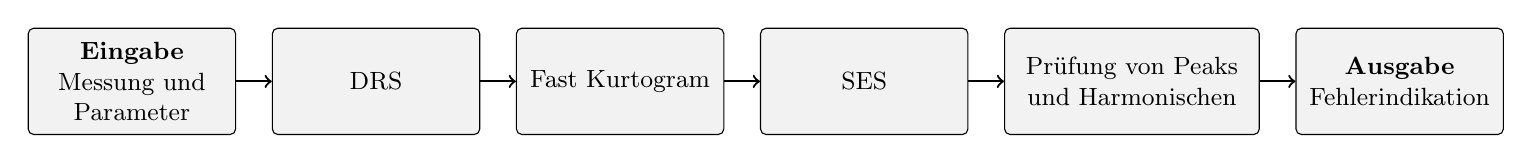
\begin{tikzpicture}[
        block/.style={
          draw,
          rounded corners=2pt,
          fill=black!5,
          align=center,
          minimum height=1.35cm,
          text width=2.4cm,
          font=\small
        }
      ]
      \node[block] (input) at (0,0)
        {\textbf{Eingabe}\\Messung und Parameter};
      \node[block] (drs) at (3.1,0) {DRS};
      \node[block] (kurtogram) at (6.2,0) {Fast Kurtogram};
      \node[block] (ses) at (9.3,0) {SES};
      \node[block, text width=3.0cm] (pruefung) at (12.7,0)
        {Prüfung von Peaks\\und Harmonischen};
      \node[block] (output) at (16.1,0)
        {\textbf{Ausgabe}\\Fehlerindikation};

      \draw[->, line width=0.8pt] (input.east) -- (drs.west);
      \draw[->, line width=0.8pt] (drs.east) -- (kurtogram.west);
      \draw[->, line width=0.8pt] (kurtogram.east) -- (ses.west);
      \draw[->, line width=0.8pt] (ses.east) -- (pruefung.west);
      \draw[->, line width=0.8pt] (pruefung.east) -- (output.west);
    \end{tikzpicture}%
  }
  \caption{Vereinfachter Datenfluss der Verarbeitungspipeline}
  \label{fig:verarbeitungspipeline_datenfluss}
  \caption*{\footnotesize Quelle: eigene Darstellung.}
\end{figure}

\paragraphheading{Fehlerindikation}
\label{par:fehlerindikation_pipeline}

Die Fehlerindikation prüft BPFO und BPFI getrennt. Für beide Frequenzen werden
die Grundfrequenz sowie die zweite und dritte Harmonische ausgewertet. Solche
Harmonischen gehören zu den erwarteten Mustern von Außen- und
Innenringschäden im \acrshort{SES}
\cite[S.~103, Tab.~1]{smithRollingElementBearing2015}.
Wie im Absatz
\hyperref[par:charakteristische_lagerschadensfrequenzen]
{\emph{Charakteristische Lagerschadensfrequenzen}} erläutert, können die
tatsächlichen Lagerfrequenzen durch Schlupf typischerweise um ein bis zwei
Prozent von den berechneten Werten abweichen
\cite[S.~487, Abschn.~1]{randallRollingElementBearing2011a}. Um solche
Abweichungen zu berücksichtigen, sucht die Entscheidungslogik um jede der drei
berechneten Frequenzen in einem relativen Fenster nach dem größten Wert des
\acrshort{SES}. Dieser Wert wird als möglicher schadensbezogener Peak weiter
geprüft. Die relative Fensterhalbbreite ist ein Entscheidungsparameter. Bei
dem in Tabelle~\ref{tab:parametrierung_suchraum} übernommenen Wert von
$1\,\%$ reicht das Suchfenster von $-1\,\%$ bis $+1\,\%$ um die berechnete
Frequenz.

Der mögliche Peak wird nicht mit einer globalen Amplitudenschwelle, sondern mit
den Werten in seiner lokalen Umgebung verglichen. Das engere Suchfenster wird
aus diesem Vergleichsbereich ausgeschlossen. Dadurch beeinflussen der zu
prüfende Peak und seine unmittelbar benachbarten Werte nicht das Niveau, mit
dem der Peak anschließend verglichen wird.

Für den lokalen Vergleich werden die Werte des \acrshort{SES} in Dezibel
umgerechnet. Proportionale Unterschiede auf der linearen Skala lassen sich
dadurch als Differenzen auswerten. Als lokales Vergleichsniveau dient der
Median. Die mediane absolute Abweichung (MAD) ist ein robustes Streuungsmaß
und wird als Median der absoluten Abstände zum Median berechnet. Da hier die
Werte des lokalen Vergleichsbereichs eingehen, beschreibt sie deren Streuung.
Für die Schwellenbildung wird die MAD mit dem in der Literatur angegebenen
Faktor $1{,}4826$ skaliert
\cite[S.~1273, Abschn.~1, Gl.~(1.2)]
{rousseeuwAlternativesMedianAbsolute1993}. Dieser Faktor ist kein anhand der
Messdaten bestimmter Entscheidungsparameter. Sofern die skalierte MAD größer
als null ist, besteht ein Peak die lokale Prüfung, wenn sein Abstand zum
Median mindestens dem durch den Parameter $k$ festgelegten Vielfachen der
skalierten MAD entspricht.

Ein Außen- oder Innenringschaden wird angezeigt, wenn die lokale Prüfung an der
zugehörigen Grundfrequenz und an mindestens einer der beiden betrachteten
Harmonischen positiv ist. Da BPFO und BPFI getrennt ausgewertet werden, kann
das Ergebnis keinen, einen oder beide Schäden enthalten. Sind beide Prüfungen
negativ, wird das Ergebnis für die Evaluation als \enquote{fehlerfrei}
behandelt. Dies bedeutet nur, dass die Regel keinen Außen- oder
Innenringschaden angezeigt hat; andere Schäden werden nicht ausgeschlossen.

Die Auswahl von BPFO, BPFI und ihren Harmonischen folgt den beschriebenen
Mustern im \acrshort{SES}. Die genaue Verknüpfung der Peaks mit der
lokalen MAD-Schwelle ist dagegen eine eigene Regel für diesen Prototyp. Ihre
Eignung muss daher in der Evaluation geprüft werden; eine allgemeine Gültigkeit
wird nicht vorausgesetzt.

\paragraphheading{Module und Schnittstellen}

Auf Grundlage des zuvor beschriebenen Datenflusses wird die Pipeline in
mehrere Module gegliedert. Jedes Modul übernimmt einen abgegrenzten Teil der
Verarbeitung. Seine Schnittstelle legt fest, welche Daten es erhält und welche
Ergebnisse es ausgibt. Tabelle~\ref{tab:pipeline_schnittstellen} gibt einen
Überblick über die Module und ihre Schnittstellen.

\begin{table}[H]
  \centering
  \small
  \caption{Module und Schnittstellen der Verarbeitungspipeline}
  \label{tab:pipeline_schnittstellen}
  \begin{tabularx}{\textwidth}{|
      >{\raggedright\arraybackslash}p{3.1cm}|
      >{\raggedright\arraybackslash}X|
      >{\raggedright\arraybackslash}X|}
    \hline
    \textbf{Modul} & \textbf{Eingaben} & \textbf{Ausgaben} \\
    \hline
    Datensatzspezifischer Import &
    Messdatei und zugehörige Datensatzkonfiguration &
    Schwingungszeitreihe, Abtastrate, Drehzahl, Lagergeometrie und Verweis auf
    die Quelldatei \\
    \hline
    Signaltrennung &
    Schwingungszeitreihe, Abtastrate, Drehzahl und DRS-Parameter &
    geschätzter deterministischer Anteil und Residuum \\
    \hline
    Frequenzbandwahl &
    Residuum, Abtastrate, Zerlegungstiefe und zulässiger Suchbereich &
    Kurtogramm sowie ausgewählte Mittenfrequenz und Bandbreite \\
    \hline
    Hüllkurvenanalyse &
    Residuum, Abtastrate, Mittenfrequenz und Bandbreite &
    Frequenzachse und Werte des \acrshort{SES} \\
    \hline
    Fehlerindikation &
    \acrshort{SES}, Drehzahl, Lagergeometrie und
    Entscheidungsparameter &
    Sollfrequenzen sowie Prüfergebnisse für BPFO und BPFI einschließlich
    der betrachteten Harmonischen \\
    \hline
    Ergebnisübergabe &
    Eingangs-, Zwischen- und Endergebnisse des Verarbeitungslaufs &
    gebündelte Ergebnisse für Protokollierung, Visualisierung und Evaluation \\
    \hline
  \end{tabularx}
\end{table}

Die Ausgabe der Pipeline enthält die Fehlerindikation und die
Zwischenergebnisse der Verarbeitung. Dazu gehören das Residuum, das
Kurtogramm, das ausgewählte Frequenzband, das \acrshort{SES} und
die berechneten Sollfrequenzen. Die einzelnen Verarbeitungsschritte lassen
sich damit getrennt von der abschließenden Klassenbewertung untersuchen. Für
die spätere Auswertung werden Dateiname, Referenzklasse und
Verarbeitungsstatus in einem Protokolldatensatz gespeichert. Kann die
Verarbeitung einer Messung nicht abgeschlossen werden, enthält dieser den
Fehlerstatus und die Fehlerursache. Für diese Messung wird keine
Fehlerindikation ausgegeben. Die konkrete Umsetzung der Schnittstellen und
die Speicherung der Ergebnisse werden in
Kapitel~\ref{ch:implementierung} beschrieben.

\section{Parametrierung}
\label{sec:parametrierungsstrategie}

Die datenabhängige Parametrierung erfolgt ausschließlich anhand der in
Abschnitt~\ref{sec:untersuchungsrahmen} festgelegten Paderborner
Trainingsgruppe. Damit berücksichtigt die Parametersuche die dort
dokumentierten Zielklassen und Betriebsbedingungen, ohne Messungen der
Paderborner Evaluationsgruppe oder des CWRU-Datensatzes zu verwenden.

Der Suchraum umfasst einen Parameter der Signalaufbereitung und die drei in
Abschnitt~\ref{sec:verarbeitungspipeline_konzept} eingeführten Parameter der
Fehlerindikation. In der Implementierung bestimmt der DRS-Blockfaktor
\texttt{n\_size}, wie viele Perioden der Wellenfrequenz einen Analyseblock
bilden. Die Wellenfrequenz wird dabei als niedrigste deterministische Frequenz
angesetzt.
\texttt{tolerance} legt die relative Halbbreite des Suchfensters um die
geprüften Sollfrequenzen fest, \texttt{freq\_search\_area} die absolute
Halbbreite ihres lokalen Vergleichsbereichs. Der Faktor $k$ bestimmt den
Mindestabstand des Peaks zum lokalen Median. Dieser Abstand wird in Einheiten
der skalierten medianen absoluten Abweichung (MAD) angegeben.

Für die Festlegung der DRS-Parameter werden die Empfehlungen von Randall
herangezogen. Er empfiehlt eine Blocklänge von 10 bis 20 Perioden der
niedrigsten zu entfernenden Frequenz und nennt als Beispiel die Frequenz der
langsamsten Welle. In dieser Arbeit wird dafür die Wellenfrequenz des
untersuchten Lagers angesetzt. Der Abstand zwischen den Blöcken soll mindestens
das Dreifache der Korrelationslänge des Lagersignals betragen. Bei einem
angenommenen Schlupf von $1\,\%$ entspricht dies ungefähr 300 Perioden der
Mittenfrequenz des Demodulationsbands
\cite[S.~277, Abschn.~7.3.2]
{randallVibrationbasedConditionMonitoring2022}. Die Implementierung bildet
diesen Abstand mit dem Sicherheitsfaktor $3$ und einer Periodenzahl von $100$.

Tabelle~\ref{tab:parametrierung_suchraum} enthält sowohl die variierten
Parameterwerte als auch die Einstellungen, die während der Suche unverändert
bleiben. Zu diesen festen Einstellungen gehören die
Zerlegungstiefe des Fast Kurtogram, die DRS-Parameter zur Bestimmung des freien
Blockabstands und der zulässige Bereich der Bandauswahl. Auch die in
Abschnitt~\ref{sec:verarbeitungspipeline_konzept} festgelegte Harmonischen- und
Entscheidungsregel bleibt unverändert.

\begin{table}[htbp]
  \centering
  \caption{Suchraum und übernommene Parameterkonfiguration}
  \label{tab:parametrierung_suchraum}
  \begin{tabularx}{\textwidth}{|
      >{\footnotesize\raggedright\arraybackslash}p{4.0cm}|
      >{\footnotesize\raggedright\arraybackslash}X|
      >{\footnotesize\raggedright\arraybackslash}p{3.0cm}|}
    \hline
    \textbf{Parameter oder feste Einstellung} &
    \textbf{Variierte Werte oder feste Einstellung} &
    \textbf{Übernommener Wert} \\
    \hline
    DRS-Blockfaktor \texttt{n\_size} &
    $\{3, 5, 10, 15, 20\}$ &
    $20$ \\
    \hline
    Schwellenfaktor $k$ &
    $\{3{,}0; 3{,}5; 4{,}0; 4{,}5; 5{,}0\}$ &
    $3{,}0$ \\
    \hline
    relative Fensterhalbbreite \texttt{tolerance} &
    $\{0{,}1; 0{,}3; 1; 2\}\,\%$ &
    $1\,\%$ \\
    \hline
    lokale Halbbreite \texttt{freq\_search\_area} &
    $\{10, 20, 40\}\,\mathrm{Hz}$ &
    $10\,\mathrm{Hz}$ \\
    \hline
    Zerlegungstiefe des Fast Kurtogram \texttt{nlevel} &
    vorab auf $8$ festgelegt &
    $8$ \\
    \hline
    Feste Parameter des DRS-Blockabstands &
    Bezugsfrequenz $3000\,\mathrm{Hz}$, Sicherheitsfaktor $3$ und
    Periodenzahl $100$; jeweils vorab festgelegt &
    $3000\,\mathrm{Hz}$; $3$; $100$ \\
    \hline
    Bandauswahl der Paderborner Parametersuche &
    Mittenfrequenz von $500$ bis $10000\,\mathrm{Hz}$ und Bandbreite von
    höchstens $2000\,\mathrm{Hz}$; vorab festgelegt &
    $500$ bis $10000\,\mathrm{Hz}$; höchstens $2000\,\mathrm{Hz}$ \\
    \hline
    Harmonischen- und Entscheidungsregel &
    gemäß Abschnitt~\ref{sec:verarbeitungspipeline_konzept}; vorab
    festgelegt &
    unverändert \\
    \hline
  \end{tabularx}
\end{table}

Die Auswahl kann folglich nur die bestplatzierte Konfiguration innerhalb
dieses diskreten Suchraums bestimmen. Werte außerhalb des Rasters werden nicht
geprüft. Ebenso bleibt offen, ob eine Änderung der in
Tabelle~\ref{tab:parametrierung_suchraum} als fest gekennzeichneten
Einstellungen zu einer anderen bestplatzierten Konfiguration führen würde.

Die vollständige Gittersuche wertet jede Kombination der vorgegebenen
diskreten Parameterwerte aus. Sie kombiniert die fünf Werte des
DRS-Blockfaktors mit $5\cdot4\cdot3=60$ Konfigurationen der
Fehlerindikation. Daraus entstehen 300 Parameterkonfigurationen. Für jeden
Wert des DRS-Blockfaktors wird die
Verarbeitung bis zum SES für alle Trainingsmessungen ausgeführt. Die daraus
resultierenden Spektren werden anschließend mit jeder zugehörigen Kombination
aus Schwellenfaktor, relativer Fensterhalbbreite und lokaler Halbbreite
ausgewertet. Als Referenz dient die aus dem jeweiligen Lagercode abgeleitete
Zielklasse.

Dabei bezeichnet \gls{TP} die Zahl der richtig positiven, \gls{FP} die Zahl
der falsch positiven und \gls{FN} die Zahl der falsch negativen Zuordnungen. Für beide
Auswertungsebenen werden daraus die Präzision $P$, die Sensitivität $R$ und das
F1-Maß berechnet:
\begin{equation}
    \begin{aligned}
        P &= \frac{TP}{TP+FP}, \\
        R &= \frac{TP}{TP+FN}, \\
        F_1 &= 2\,\frac{P\,R}{P+R}.
    \end{aligned}
    \label{eq:f1_mass}
\end{equation}
Die Rangfolge wird primär nach dem F1-Maß der Klassenzuordnung gebildet. Bei
gleichem Wert entscheidet zunächst der Anteil der Messungen, deren Ausgabe
exakt nur die jeweilige Referenzklasse enthält, und danach das binäre F1-Maß
der Schadenserkennung. Weitere Gleichstände werden anhand einer festen
Reihenfolge der Parameterwerte aufgelöst. Kennwerte der späteren
Evaluationsmessungen sind kein Bestandteil dieser Rangfolge.

Die vollständige Rangliste mit den Kennwerten aller 300 Konfigurationen wird
in einer Ergebnisdatei gespeichert. Die beiden bestplatzierten Konfigurationen
stimmen in den drei vorrangigen Auswahlkennwerten überein und unterscheiden
sich nur in der relativen Fensterhalbbreite. Gemäß der festgelegten
Reihenfolge wird deshalb der kleinere Wert von $1\,\%$ übernommen. Aus der
bestplatzierten Zeile werden die Zerlegungstiefe, die Bezugsfrequenz, der
DRS-Blockfaktor und die drei Parameter der Fehlerindikation geladen. Der
Sicherheitsfaktor $3$ und die Periodenzahl $100$ stehen nicht in der Rangliste,
sondern sind in der Ladefunktion fest hinterlegt. Der daraus gebildete
Parametersatz wird für die Paderborner sowie die zusätzliche CWRU-Evaluation
verwendet. Abtastrate, Lagergeometrie und der datensatzspezifische Bereich der
Bandauswahl werden separat bereitgestellt und sind nicht in dieser
Ranglistendatei gespeichert. Tabelle~\ref{tab:parametrierung_suchraum} nennt die
übernommene Parameterkonfiguration. Die zugehörigen F1-Werte und weiteren Kennzahlen der
Parametersuche werden erst in Abschnitt~\ref{sec:pipelineergebnisse} als
Ergebnis der Parameterstudie dargestellt.

\section{Evaluationskonzept}
\label{sec:evaluationskonzept}

Das Evaluationskonzept baut auf dem methodischen Vorgehen aus
Abschnitt~\ref{sec:methodisches_vorgehen} auf und legt fest, wie die entwickelte
Pipeline untersucht und bewertet wird. Es umfasst die Prüfung einzelner
Softwarekomponenten, die Bewertung der vollständigen Pipeline anhand von
Messungen, die nicht zur Parametrierung verwendet wurden, sowie den Vergleich
der Fehlerindikationen mit und ohne Signaltrennung. Da die Auswahl der Daten
und die Trennung von Parametrierung und Evaluation bereits in
Abschnitt~\ref{sec:untersuchungsrahmen} festgelegt wurden, beschreibt dieser
Abschnitt, welche Komponenten geprüft, welche Pipelinekonfigurationen verglichen
und wie die Ergebnisse ausgewertet werden. Die Durchführung der Versuche und
die Ergebnisse werden in
Kapitel~\ref{ch:evaluation} dargestellt.

\paragraphheading{Komponentenvalidierung}

Die \gls{DRS} wird zunächst unabhängig von der nachfolgenden Auswahl des
Frequenzbandes und der Fehlerindikation geprüft. Bei der Vorbereitung des Tests
wurde weder eine unabhängige DRS-Implementierung mit Referenzausgaben noch ein
öffentlich zugänglicher Datensatz gefunden, in dem der deterministische und
der zufällige Signalanteil getrennt vorgegeben sind. Deshalb werden die
Testsignale selbst erzeugt; ihre beiden Anteile sind bereits vor der Mischung
bekannt.

Der deterministische Referenzanteil besteht aus mehreren Sinusschwingungen.
Der zufällige Referenzanteil setzt sich aus weißem Rauschen und einer
Impulsfolge zusammen, deren Abstände und Amplituden variiert werden. Die
Impulsfolge regt eine abklingende Resonanz an. Der von der \gls{DRS} geschätzte
deterministische Anteil wird mit dem deterministischen Referenzanteil
verglichen, das Residuum mit dem zufälligen Referenzanteil. Bewertet werden die
Korrelation und der \gls{RMSE} zwischen Schätzung und Referenz. Der
\gls{RMSE} ist die Quadratwurzel der mittleren quadrierten Abweichung. Damit Signale
unterschiedlicher Stärke vergleichbar bleiben, wird er durch den Effektivwert
des Referenzanteils geteilt. Zusätzlich wird das Verhältnis der Effektivwerte
von Schätzung und Referenz angegeben. Der Effektivwert wird dabei als
\gls{RMS} berechnet. Weiterhin wird geprüft, ob die Summe
beider Ausgangssignale das Eingangssignal rekonstruiert und ob ein
ausschließlich aus weißem Rauschen bestehendes Eingangssignal weitgehend im
Residuum erhalten bleibt.

\newpage
Für $N$ Abtastwerte bezeichnen $x_i$ die Referenz und $\hat{x}_i$ die
Schätzung; $\bar{x}$ und $\overline{\hat{x}}$ sind ihre arithmetischen
Mittelwerte. Für den Rekonstruktionsfehler steht $s_i$ für das Eingangssignal,
$\hat{d}_i$ für den geschätzten deterministischen Anteil und $\hat{z}_i$ für
das Residuum. Die verwendeten Kennwerte sind wie folgt definiert:
\begin{equation}
    \begin{aligned}
        \operatorname{RMSE}(x,\hat{x})
            &= \sqrt{\frac{1}{N}\sum_{i=1}^{N}(x_i-\hat{x}_i)^2}, \\
        \operatorname{RMS}(x)
            &= \sqrt{\frac{1}{N}\sum_{i=1}^{N}x_i^2}, \\
        \operatorname{RMSE}_{\mathrm{norm}}(x,\hat{x})
            &= \frac{\operatorname{RMSE}(x,\hat{x})}{\operatorname{RMS}(x)}, \\
        q_{\mathrm{RMS}}(x,\hat{x})
            &= \frac{\operatorname{RMS}(\hat{x})}{\operatorname{RMS}(x)}, \\
        \rho(x,\hat{x})
            &= \frac{\sum_{i=1}^{N}(x_i-\bar{x})(\hat{x}_i-\overline{\hat{x}})}
                    {\sqrt{\sum_{i=1}^{N}(x_i-\bar{x})^2
                    \sum_{i=1}^{N}(\hat{x}_i-\overline{\hat{x}})^2}}, \\
        e_{\mathrm{rec}}
            &= \max_{1\leq i\leq N}\left|s_i-\hat{d}_i-\hat{z}_i\right|.
    \end{aligned}
    \label{eq:komponentenvalidierung_kennwerte}
\end{equation}

Um nicht nur ein einziges Signal zu prüfen, wird der Test mit mehreren Varianten
wiederholt. Zwischen den Varianten ändern sich der Zufallsstartwert, die
Rauschstärke und die Frequenz einer deterministischen Komponente.

Die im Prototyp verwendete Fast-Kurtogram-Implementierung basiert auf einer von
T.~Lecocq für Waveloc erstellten Python-2-Übertragung von Antonis MATLAB-Code
\cite{lecocqFastKurtogram2012}.
Für diese Arbeit wurde sie an Python~3 angepasst und weiter überarbeitet. Da
die verwendete Fassung damit sowohl vom MATLAB-Original als auch von der
übernommenen Python-Fassung abweicht, werden ihre Ergebnisse mit Antonis
originaler MATLAB-Implementierung des Fast Kurtogram verglichen.

Beide Programme verarbeiten dieselbe Auswahl Paderborner Messsignale mit
derselben Abtastrate und Zerlegungstiefe. Für jedes Signal werden die gewählte
Mittenfrequenz, die Bandbreite und alle Werte der Kurtogrammmatrix verglichen.
Als relative Toleranz wird $10^{-6}$ und als absolute Toleranz $10^{-8}$
verwendet. Diese engen Grenzen lassen nur sehr kleine numerische Abweichungen
zu, wie sie etwa durch Gleitkomma-Rundungen entstehen können. Zusätzlich werden
für Mittenfrequenz und Bandbreite die mittleren
absoluten Abweichungen erfasst. Für die Matrixwerte werden die mittlere absolute
Abweichung, der \gls{RMSE} und die Korrelation protokolliert. Der \gls{RMSE}
und die Korrelation werden dabei nach
Gleichung~\eqref{eq:komponentenvalidierung_kennwerte} berechnet. Die Ergebnisse
werden in Abschnitt~\ref{sec:komponentenvalidierung} berichtet.

Die Komponentenprüfung umfasst außerdem die Berechnung der Sollfrequenzen und
die regelbasierte Spektrumauswertung. Die für Innen- und Außenringschäden
berechneten Sollfrequenzen werden mit unabhängig bestimmten Referenzwerten für
festgelegte Drehzahlen und Lagergeometrien verglichen. Die Entscheidungslogik
wird mit künstlichen Spektren geprüft. Darin liegen Peaks an den
Sollfrequenzen und ihren Harmonischen gezielt innerhalb oder außerhalb der
festgelegten Suchfenster sowie oberhalb oder unterhalb der Schwellenwerte. Die
Prüfung umfasst mindestens vier Fälle: keine Erkennung, ausschließlich eine
Innenringerkennung, ausschließlich eine Außenringerkennung und die
gleichzeitige Erkennung beider Fehlerarten.

\paragraphheading{Pipelineevaluation}
\label{par:pipelineevaluation}

Für beide Evaluationen werden die Parameter verwendet, die zuvor mit den
Paderborner Trainingsdaten bestimmt wurden. Zunächst wird die Pipeline mit
der getrennten Paderborner Evaluationsgruppe geprüft. Dieser Lauf untersucht
real entstandene Schäden an Lagern, die nicht für die Parametrierung verwendet
wurden. Danach werden dieselben Parameter auf die ausgewählten CWRU-Messungen
angewendet. Die Kennwerte beider Läufe werden getrennt ausgewiesen und nicht
zu einem gemeinsamen Gesamtergebnis zusammengefasst.

Um den Beitrag der Signaltrennung zu untersuchen, werden zwei Varianten der
Pipeline verglichen. Die erste Variante verwendet das \gls{DRS}-Residuum für
das Fast Kurtogram und die Hüllkurvenanalyse. Die zweite Variante überspringt
die Signaltrennung und verarbeitet stattdessen das Rohsignal. Datenauswahl,
Lagergeometrie, Abtastrate, Frequenzband und alle weiteren Parameter bleiben
gleich. Beide Varianten werden auf dieselben Messaufzeichnungen angewendet.
Der Vergleich zeigt daher nur den Beitrag der \gls{DRS} innerhalb der
entwickelten Pipeline. Eine Überlegenheit gegenüber anderen
Diagnoseverfahren lässt sich daraus nicht ableiten.

Jede Messaufzeichnung wird einzeln ausgewertet. Die Skripte erfassen für jeden
Lauf, wie viele Dateien übergeben, erfolgreich verarbeitet oder mit einem
Fehler abgebrochen wurden. Für Paderborn wird zusätzlich geprüft, ob für jedes
ausgewählte Lager die erwartete Anzahl an Aufzeichnungen vorhanden ist. Eine
Aufzeichnung geht nur dann in die Kennzahlen ein, wenn ihre Verarbeitung mit
dem Status \texttt{ok} abgeschlossen wurde. Bei fehlgeschlagenen Dateien wird
die Ursache protokolliert. Ihre Anzahl wird zusammen mit der Zahl der
übergebenen und der erfolgreich verarbeiteten Dateien angegeben.

\paragraphheading{Bewertungskennzahlen}

Gemäß Anforderung E-03 im Absatz
\hyperref[par:festlegungen_evaluation]{\enquote{Festlegungen für die
Evaluation}} wird die Bewertung in zwei Ebenen unterteilt: die binäre
Schadenserkennung und die Klassenzuordnung des Lagerzustands.

Für die Schadenserkennung wird jede Messung binär ausgewertet. Eine
Referenzmessung gilt als geschädigt, wenn ihr ein Innen- oder
Außenringschaden zugeordnet ist. Andernfalls gilt sie als fehlerfrei. Auf
Ausgabeseite gilt ein Schaden als erkannt, sobald die Pipeline mindestens eine
Innen- oder Außenringindikation meldet. Ohne eine solche Meldung lautet die
Ausgabe \enquote{fehlerfrei}. Aus dem Vergleich von Referenz und Ausgabe
entstehen die Zählwerte \gls{TP}, \gls{TN}, \gls{FP} und \gls{FN}. Daraus
werden Präzision, Sensitivität, Spezifität, Fehlalarmrate, Genauigkeit und
F1-Maß berechnet.

Bei der Diagnose wird für jede Messung festgehalten, welche Klassen die
Pipeline erkannt hat. Innen- und Außenringindikationen können dabei
gleichzeitig vorliegen. Jede erfolgreich ausgewertete Messaufzeichnung besitzt
genau eine Referenzklasse. Enthält das Ergebnis diese Klasse, wird eine richtige
Zuordnung gezählt und \gls{TP} erhöht. Jede zusätzlich erkannte Klasse erhöht
\gls{FP}. Fehlt die Referenzklasse im Ergebnis, wird dies als Auslassung erfasst
und \gls{FN} erhöht. Ein \gls{TN} wird bei der Klassenzuordnung nicht gebildet,
da für eine Messung mehrere nicht zutreffende Klassen vorliegen und ein
gemeinsamer TN-Zählwert daher nicht eindeutig wäre. Für Präzision,
Sensitivität und F1-Maß werden nur \gls{TP}, \gls{FP} und \gls{FN} benötigt.
Diese Kennzahlen werden aus den
über alle erfolgreich ausgewerteten Aufzeichnungen kumulierten Zählwerten
berechnet. Ergänzend wird
der Anteil exakt richtiger Zuordnungen ausgewiesen. Eine Zuordnung gilt genau
dann als exakt, wenn das Ergebnis ausschließlich die Referenzklasse enthält.
Damit wird zwischen einer eindeutigen richtigen Ausgabe und einer Ausgabe mit
zusätzlicher Fehlerindikation unterschieden.

Die Ergebniszusammenfassungen enthalten für die binäre Schadenserkennung die
Zählwerte \gls{TP}, \gls{TN}, \gls{FP} und \gls{FN}. Für die
Klassenzuordnung werden dagegen \gls{TP}, \gls{FP} und \gls{FN} gespeichert.
Zusätzlich werden die Zahl der übergebenen und erfolgreich ausgewerteten
Aufzeichnungen sowie die Zahl fehlgeschlagener Verarbeitungen angegeben. Die
Kennzahlen werden für den Paderborner und den CWRU-Datensatz getrennt
ausgewiesen.

Für den im Absatz
\hyperref[par:pipelineevaluation]{\enquote{Pipelineevaluation}} beschriebenen
Vergleich werden die Kennzahlen für beide Varianten getrennt ausgewiesen. Ein
einzelner zusammengefasster
Kennwert bildet nicht die alleinige Grundlage für die Beurteilung der Pipeline.
Die Beurteilung berücksichtigt die Schadenserkennung, die Klassenzuordnung und
die in Abschnitt~\ref{sec:fehleranalyse} untersuchten Fehlermuster.
